
\section*{descrição do problema}

Este trabalho visa apresentar o comparativo entre ao menos dois destes três algoritmos, apresentando tempo de execução e taxa de precisão de rostos. Espera-se como resultados que o software seja estável, consiga identificar rostos em uma imagem e possa destaca-los para a apresentação de resultados.

\section*{estado da arte}

% http://www.linhadecodigo.com.br/artigo/1813/biometria-reconhecimento-facial-livre.aspx
Um dos processos de identificação mais utilizados pelos seres humanos é o reconhecimento facial, o qual permite identificar rapidamente qualquer pessoa e assim definir o tipo apropriado de interação com ela. O reconhecimento facial ainda nos oferece a possibilidade de perceber o estado emocional de uma pessoa, contribuindo para o relacionamento.

O reconhecimento facial é extremamente complexo de implementar em uma máquina, visto não sabermos ao certo como o cérebro humano realiza essa tarefa. O cérebro humano pode identificar corretamente uma pessoa a partir de sua imagem facial mesmo sobre as mais diversas condições, como variações de iluminação, observando apenas uma de suas características ou partes, e até mesmo com distorções ou deformações.

% http://docs.opencv.org/2.4/modules/contrib/doc/facerec/facerec_tutorial.html
O reconhecimento de faces baseado na geometria do rosto é a abordagem mais intuitiva para este tipo de reconhecimento. Um dos primeiros sistemas automatizados para isso é descrito em \cite{kanade1973picture}: pontos chaves (posição dos olhos, orelhas e nariz, por exemplos) são utilizados para definir um vetor de características entre estes pontos (distâncias e ângulos entre eles). O reconhecimento ocorre calculando as distâncias euclidianas entre os pontos e uma imagem de referência. Tal método é robusto contra variações de iluminação, porém possui um grande problema: o exato registro de pontos chave é complexo mesmo com algoritmos do estado da arte. Algum dos últimos trabalhos em reconhecimento geométrico de faces realizado em \cite{brunelli1992face}. Experimentos em grandes conjuntos de dados utilizado um vetor de características de 22 dimensões mostraram que o reconhecimento geométrico sozinho não contém informação suficiente para realizar um reconhecimento adequado.
%Face recognition based on the geometric features of a face is probably the most intuitive approach to face recognition. One of the first automated face recognition systems was described in \cite{kanade1973picture}: marker points (position of eyes, ears, nose, ...) were used to build a feature vector (distance between the points, angle between them, ...). The recognition was performed by calculating the euclidean distance between feature vectors of a probe and reference image. Such a method is robust against changes in illumination by its nature, but has a huge drawback: the accurate registration of the marker points is complicated, even with state of the art algorithms. Some of the latest work on geometric face recognition was carried out in \cite{brunelli1992face}. A 22-dimensional feature vector was used and experiments on large datasets have shown, that geometrical features alone my not carry enough information for face recognition.

O método Eingenfaces descrito em \cite{eigenfaces} tomou um abordagem holística para o reconhecimento facial: Uma imagem facial é um ponto multidimensional no qual é determinado uma representação em menos dimensões para facilitar a classificação. A representação em menos dimensões é feita utilizando a Análise de Componentes Principais (PCA, em inglês) que identifica os eixos com maior variação. Contudo, enquanto esta transformação é ótima para a reconstrução de pontos ela não leva em conta as classes da imagem. Por exemplo, se a variação é gerada por uma fonte como a luz, o eixo com maior variação não necessariamente contém informações características sobre a fonte de tal forma que uma classificação de torna impossível. Para contornar o problema uma projeção específica de classe com \textit{Linear Discriminat Analysis} foi aplicada em \cite{fisherfaces}. A ideia é minimizar a variação em uma classe enquanto maximiza-se a variação entre classes ao mesmo tempo.
%The Eigenfaces method described in \cite{eigenfaces} took a holistic approach to face recognition: A facial image is a point from a high-dimensional image space and a lower-dimensional representation is found, where classification becomes easy. The lower-dimensional subspace is found with Principal Component Analysis, which identifies the axes with maximum variance. While this kind of transformation is optimal from a reconstruction standpoint, it doesn’t take any class labels into account. Imagine a situation where the variance is generated from external sources, let it be light. The axes with maximum variance do not necessarily contain any discriminative information at all, hence a classification becomes impossible. So a class-specific projection with a Linear Discriminant Analysis was applied to face recognition in \cite{fisherfaces}. The basic idea is to minimize the variance within a class, while maximizing the variance between the classes at the same time.

Recentemente diversos métodos para reconhecimento de características faciais surgiram. Para evitar a grande quantidade de dimensões nos dados de entrada apenas certas regiões de uma imagem são descritas. Espera-se que as características utilizadas sejam mais robustas contra obstrução, iluminação e quantidades pequenas de amostras. Algorítimos utilizados para obtenção de características locais são: Gabor Wavelets \cite{wiskott1997face}, transformada discreta de cossenos \cite{messer2006performance} e padrões binários locais \cite{binaryface}. A melhor maneira de preservar informação espacial ao aplicar um método de obtenção local ainda é uma questão aberta para pesquisa, pois a informação espacial é potencialmente útil.
%Recently various methods for a local feature extraction emerged. To avoid the high-dimensionality of the input data only local regions of an image are described, the extracted features are (hopefully) more robust against partial occlusion, illumation and small sample size. Algorithms used for a local feature extraction are Gabor Wavelets \cite{wiskott1997face}, Discrete Cosinus Transform \cite{messer2006performance} and Local Binary Patterns \cite{binaryface}. It’s still an open research question what’s the best way to preserve spatial information when applying a local feature extraction, because spatial information is potentially useful information.

\section*{abordagem escolhida}

% http://docs.opencv.org/2.4/modules/contrib/doc/facerec/facerec_tutorial.html
Hoje a biblioteca OpenCV oferece três algoritmos de reconhecimento facial disponíveis para uso gratuito. 
% https://github.com/bytefish/facerec
\subsection*{Eigenfaces} % (fold)
\label{sub:eigenfaces}

% Turk, M., and Pentland, A. "Eigenfaces for recognition.". Journal of Cognitive Neuroscience 3 (1991), 71–86.
A grande quantidade de dimensões é o problema com as represetações de imagens. Imagens em $p \times q$ tons de cinza produzem um vetor $m = pq$-dimensional espacial, logo uma imagem com $100 \times 100$ pixels possui um vetor 10,000-dimensional espacial. A questão é: todas estas dimensões são úteis? Só é possível tomar uma decisão se houver uma variação nos dados, então é preciso encontrar os componentes que contém maior informação. A Análise de Componentes Principais (PCA, em inglês) foi proposta independentemente por Karl Pearson (1901) e Harold Hotelling (1933) para transformar um conjunto de possíveis variáveis correlacionadas em um conjunto menor de variáveis não correlacionadas. A ideia por trás disso é que um conjunto multidimensional de variáveis é frequentemente descrito por um conjunto de variáveis correlacionadas, logo apenas algumas dimensões são responsáveis pela maior parte das informações. O método PCA encontra as direções com maior variação de dados, chamados de componentes principais.
%The problem with the image representation we are given is its high dimensionality. Two-dimensional $p \times q$ grayscale images span a $m = pq$-dimensional vector space, so an image with $100 \times 100$ pixels lies in a 10,000-dimensional image space already. The question is: Are all dimensions equally useful for us? We can only make a decision if there’s any variance in data, so what we are looking for are the components that account for most of the information. The Principal Component Analysis (PCA) was independently proposed by Karl Pearson (1901) and Harold Hotelling (1933) to turn a set of possibly correlated variables into a smaller set of uncorrelated variables. The idea is, that a high-dimensional dataset is often described by correlated variables and therefore only a few meaningful dimensions account for most of the information. The PCA method finds the directions with the greatest variance in the data, called principal components.

\subsubsection*{Descrição do Algoritmo} % (fold)

Sendo $X = \{ x_{1}, x_{2}, \ldots, x_{n} \}$ tal que $x_i \in R^{d}$.

\begin{enumerate}
    \item Calcule a média $\mu$.

    \begin{equation*}
        \mu = \frac{1}{n} \sum_{i=1}^{n} x_{i}
    \end{equation*}
    \item Calcule a matriz de covariância $S$.

    \begin{equation*}
        S = \frac{1}{n} \sum_{i=1}^{n} (x_{i} - \mu) (x_{i} - \mu)^{T}`
    \end{equation*}

    \item Calcule os autovalores $\lambda_{i}$ e autovetores $v_{i}$ de $S$.

    \begin{equation*}
        S v_{i} = \lambda_{i} v_{i}, i=1,2,\ldots,n
    \end{equation*}

    \item Os $k$ principais componentes são os autovetores correspondentes aos $k$ maiores autovalores, dados por:

    \begin{equation*}
        y = W^{T} (x - \mu)
    \end{equation*}

    Sendo $W = (v_{1}, v_{2}, \ldots, v_{k})$.

    \item Sendo o PCA dado por: $x = W y + \mu$,
    \begin{itemize}
        \item Projeta-se todas as amostras de treinamento no subespaço PCA.
        \item Projeta-se a imagem de analise no subespaço PCA.
        \item Localize os vizinhos mais próximos entre as imagens de treinamento e a imagem de analise.
    \end{itemize}
\end{enumerate}

Os autovetores resultantes são ortogonais. Para adquirir os autovetores ortonormais é necessário normaliza-los.

% subsubsection algoritmo (end)

\subsection*{Fisherfaces} % (fold)
\label{sub:fisherfaces}

% Belhumeur, P. N., Hespanha, J., and Kriegman, D. "Eigenfaces vs. Fisherfaces: Recognition using class specific linear projection.". IEEE Transactions on Pattern Analysis and Machine Intelligence 19, 7 (1997), 711–720.
A Análise Discriminante Linear (LDA, em inglês) executa uma redução dimensional específica de classe e foi inventada pelo renomado estatístico Sir R. A. Fisher. Ele utilzou com êxito esta análise para classificar flores em sua tese de 1936 ``The use of multiple measurements in taxonomic problems'' \cite{fisher1936use}. Para encontrar a combinação ótima de características que melhor separam as  classes a LDA maximiza a dispersão da razão entre-classes e inter-classes ao invés de maximizar a dispersão geral. A ideia é simples: as mesmas classes devem se agrupar fortemente juntas enquanto classes diferentes devem estar tão distantes quanto possível nas representação com poucas dimensões. Isto foi percebido também por Belhumeur, Hespanha e Kriegman e então eles aplicaram a análise discriminante para o reconhecimento de faces em \cite{fisherfaces}.
%The Linear Discriminant Analysis performs a class-specific dimensionality reduction and was invented by the great statistician Sir R. A. Fisher. He successfully used it for classifying flowers in his 1936 paper The use of multiple measurements in taxonomic problems \cite{fisher1936use}. In order to find the combination of features that separates best between classes the Linear Discriminant Analysis maximizes the ratio of between-classes to within-classes scatter, instead of maximizing the overall scatter. The idea is simple: same classes should cluster tightly together, while different classes are as far away as possible from each other in the lower-dimensional representation. This was also recognized by Belhumeur, Hespanha and Kriegman and so they applied a Discriminant Analysis to face recognition in \cite{fisherfaces}.
% \citeonline{fisherfaces}.

\subsubsection*{Descrição do Algoritmo} % (fold)

Sendo $X$ um conjunto de classes $X  = \{X_1,X_2,\ldots,X_c\}$ tal que  $X_i  = \{x_1, x_2, \ldots, x_n\}$ e suas matrizes de dispersão  $S_{B}$ e $S_{W}$ sendo dadas como:

\begin{align*} 
    S_{B} = & \sum_{i=1}^{c} N_{i} (\mu_i - \mu)(\mu_i - \mu)^{T} \\ 
    S_{W} = & \sum_{i=1}^{c} \sum_{x_{j} \in X_{i}} (x_j - \mu_i)(x_j - \mu_i)^{T} 
\end{align*}

Sendo $\mu$ a média total e $\mu_i$ a média da classe $i \in \{1,\ldots,c\}$.

O algoritmo de Fisher procura pela projeção $W$ que máximiza a separação de classes, dada por:

\begin{equation*}
W_{opt} = \operatorname{arg\,max}_{W} \frac{|W^T S_B W|}{|W^T S_W W|}
\end{equation*}

Segundo \cite{fisherfaces} a otimização para essa solução é data pela resolução do problema geral de autovalores:



\begin{align*} 
    S_{B} v_{i} = & \lambda_{i} S_w v_{i} \nonumber \\ 
    S_{W}^{-1} S_{B} v_{i} = & \lambda_{i} v_{i} 
\end{align*}


\subsection*{Local Binary Patterns Histograms} % (fold)
\label{sub:local_binary_patterns_histograms}

% Ahonen, T., Hadid, A., and Pietikainen, M. "Face Recognition with Local Binary Patterns.". Computer Vision - ECCV 2004 (2004), 469–481.
A ideia não é olhar para toda uma figura como um vetor multidimensional, mas para descrever apenas características locais de um objeto. As características que são obtidas desta maneira vão possuir, implicitamente, menos dimensões. Uma ótima ideia,  porém será observado que a representação que é recebida não sofre apenas com a variação de iluminação. Outros problemas como variação de escala, rotação e translação em imagens - a descrição local deve ser robusta contra estes problemas. Assim como {\ttfamily SIFT}, a metodologia do Local Binary Pattern (LBP) se originou da análise de texturas 2D. A ideia básica do LBP é resumir a estrutura local de uma imagem comparando cada pixel com o seu vizinho. Definindo os pixels vizinhos a um central como limitantes é possível avaliar a intensidade entre eles, se o pixel central possuir intensidade maior ou igual aos vizinhos então este é designado como 1, caso o contrário o pixel central é designado como 0. Por fim restará uma representação binária para cada pixel, assim como {\ttfamily 11001111}. Com uma vizinhança de 8 pixels haverá $2^8$ possíveis combinações chamadas de Local Binarry Patterns, ou códigos LBP. O primeiro operador LBP descrito utilizava uma vizinhança $3 \times 3$ fixa.

 %The idea is to not look at the whole image as a high-dimensional vector, but describe only local features of an object. The features you extract this way will have a low-dimensionality implicitly. A fine idea! But you’ll soon observe the image representation we are given doesn’t only suffer from illumination variations. Think of things like scale, translation or rotation in images - your local description has to be at least a bit robust against those things. Just like {\ttfamily SIFT}, the Local Binary Patterns methodology has its roots in 2D texture analysis. The basic idea of Local Binary Patterns is to summarize the local structure in an image by comparing each pixel with its neighborhood. Take a pixel as center and threshold its neighbors against. If the intensity of the center pixel is greater-equal its neighbor, then denote it with 1 and 0 if not. You’ll end up with a binary number for each pixel, just like {\ttfamily 11001111}. So with 8 surrounding pixels you’ll end up with $2^8$ possible combinations, called Local Binary Patterns or sometimes referred to as LBP codes. The first LBP operator described in literature actually used a fixed $3 \times 3$ neighborhood.

\subsubsection*{Descrição do Algoritmo} % (fold)

Uma descrição mais formal do operador de LBP pode ser dada como:
$LBP(x_c, y_c) = \sum_{p=0}^{P-1} 2^p s(i_p - i_c)$
com $(x_c, y_c)$ como pixel central de intensidade $i_c$, e $i_n$ como a intensidade do pixel vizinho. $s$ é o sinal da função definido como:
\begin{equation*} s(x) = \begin{cases} 1 & \text{if $x \geq 0$}\\ 0 & \text{else} \end{cases} \end{equation*}
Essa descrição permite capturar detalhes bem finos da imagem. Na verdade, os autores foram capazes de competir com resultados inovadores de classificação de texturas. Logo após a publicação do operados, verificou-se que uma vizinhança fixa falha ao codificar detalhes que diferem em escala. Assim, o operador foi extendido para usar uma vizinhança variável em \cite{binaryface}. A idéia é alinhar um número arbitrário de vizinhos em um círculo com um raio variável que permite capturar as seguintes vizinhanças:

% \end{multicols*}
% \begin{figure}[h]
% \centering
    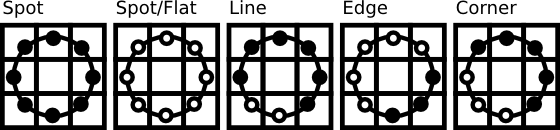
\includegraphics[width=0.45\textwidth]{conteudo/patterns}
    % \caption{}
    % \label{radius}
% \end{figure}
% \begin{multicols*}{2} 

Para um dado ponto $(x_c, y_c)$, a posição do vizinho $(x_p,y_p), p \in P$ pode ser calculado por:
\begin{align*}
x_{p} & = x_c + R \cos({\frac{2\pi p}{P}})\\
y_{p} & = y_c - R \sin({\frac{2\pi p}{P}})
\end{align*}
Onde $R$ é o raio e $P$ é o número de pontos de amostragem.
O operador é uma extensão para os códigos originais LBP, por isso algumas vezes ele é chamado LBP Extendido (também referido com LBP Circular). Se uma coordenada de pontos sobre o círculo não corresponde às coordenadas da imagem, ela é interpolada. ciência da computação tem um monte de esquemas de interpolação inteligentes , a implementação OpenCV faz uma interpolação bilinear:
\begin{align*}
f(x,y) \approx \begin{bmatrix}
    1-x & x \end{bmatrix} \begin{bmatrix}
    f(0,0) & f(0,1) \\
    f(1,0) & f(1,1) \end{bmatrix} \begin{bmatrix}
    1-y \\
    y \end{bmatrix}
\end{align*}

\section*{resultados e simulações}

% \lipsum[4]

\section*{conclusões e trabalhos futuros}

O algoritmo de Eigenvectors possui alguns benefícios, como capturar a iluminação , porém  são necessárias uma grande quantidade de imagens para se alcançar um resultado considerável. Já o algoritmo de Fisherfaces consegue convergir para resultados palpáveis com menos imagens, porém seus resultados são muito sensíveis com a iluminação.

Por obter resultados em menos iterações, o algoritmo de Fisherfaces é interessante para propostas de localização de rostos ou olhos, como para substituição de características ou aplicação de mascaras como no aplicativo Snapchat. Porém, para aplicações no intuito de reconhecimento, como desbloqueio de tela ou controle de acesso presencial empresarial o Eigenvectors se mostra mais interessante, visto ser menos suscetível a falhas por questão de iluminação.

% \lipsum[5]
